% Options for packages loaded elsewhere
\PassOptionsToPackage{unicode}{hyperref}
\PassOptionsToPackage{hyphens}{url}
\PassOptionsToPackage{dvipsnames,svgnames,x11names}{xcolor}
%
\documentclass[
  12pt,
]{article}
\usepackage{amsmath,amssymb}
\usepackage{lmodern}
\usepackage{iftex}
\ifPDFTeX
  \usepackage[T1]{fontenc}
  \usepackage[utf8]{inputenc}
  \usepackage{textcomp} % provide euro and other symbols
\else % if luatex or xetex
  \usepackage{unicode-math}
  \defaultfontfeatures{Scale=MatchLowercase}
  \defaultfontfeatures[\rmfamily]{Ligatures=TeX,Scale=1}
\fi
% Use upquote if available, for straight quotes in verbatim environments
\IfFileExists{upquote.sty}{\usepackage{upquote}}{}
\IfFileExists{microtype.sty}{% use microtype if available
  \usepackage[]{microtype}
  \UseMicrotypeSet[protrusion]{basicmath} % disable protrusion for tt fonts
}{}
\makeatletter
\@ifundefined{KOMAClassName}{% if non-KOMA class
  \IfFileExists{parskip.sty}{%
    \usepackage{parskip}
  }{% else
    \setlength{\parindent}{0pt}
    \setlength{\parskip}{6pt plus 2pt minus 1pt}}
}{% if KOMA class
  \KOMAoptions{parskip=half}}
\makeatother
\usepackage{xcolor}
\usepackage[margin=1in]{geometry}
\usepackage{longtable,booktabs,array}
\usepackage{calc} % for calculating minipage widths
% Correct order of tables after \paragraph or \subparagraph
\usepackage{etoolbox}
\makeatletter
\patchcmd\longtable{\par}{\if@noskipsec\mbox{}\fi\par}{}{}
\makeatother
% Allow footnotes in longtable head/foot
\IfFileExists{footnotehyper.sty}{\usepackage{footnotehyper}}{\usepackage{footnote}}
\makesavenoteenv{longtable}
\usepackage{graphicx}
\makeatletter
\def\maxwidth{\ifdim\Gin@nat@width>\linewidth\linewidth\else\Gin@nat@width\fi}
\def\maxheight{\ifdim\Gin@nat@height>\textheight\textheight\else\Gin@nat@height\fi}
\makeatother
% Scale images if necessary, so that they will not overflow the page
% margins by default, and it is still possible to overwrite the defaults
% using explicit options in \includegraphics[width, height, ...]{}
\setkeys{Gin}{width=\maxwidth,height=\maxheight,keepaspectratio}
% Set default figure placement to htbp
\makeatletter
\def\fps@figure{htbp}
\makeatother
\setlength{\emergencystretch}{3em} % prevent overfull lines
\providecommand{\tightlist}{%
  \setlength{\itemsep}{0pt}\setlength{\parskip}{0pt}}
\setcounter{secnumdepth}{5}
\usepackage{setspace} \setstretch{1.15} \usepackage{float} \floatplacement{figure}{t}
\ifLuaTeX
  \usepackage{selnolig}  % disable illegal ligatures
\fi
\IfFileExists{bookmark.sty}{\usepackage{bookmark}}{\usepackage{hyperref}}
\IfFileExists{xurl.sty}{\usepackage{xurl}}{} % add URL line breaks if available
\urlstyle{same} % disable monospaced font for URLs
\hypersetup{
  colorlinks=true,
  linkcolor={cyan},
  filecolor={Maroon},
  citecolor={Blue},
  urlcolor={cyan},
  pdfcreator={LaTeX via pandoc}}

\title{~\Large Indian Premier League Cricket}
\author{\large Matt Stuart\(^{1,2}\), Hassan Raffique\(^{3}\), Leigha
DeRango\(^1\)\\
\large Gregory J. Matthews\(^{1,2}\)\\
\vspace{-1.1mm}\\
\large \(^1\) Department of Mathematics and Statistics, Loyola
University Chicago, Chicago, IL, USA \vspace{-1.1mm}\\
\large \(^2\) Center for Data Science and Consulting, Loyola University
Chicago, Chicago, IL, USA \vspace{-1.1mm}\\
\large \(^3\) Univsersiry of Iowa, Iowa City, IA \vspace{-1.1mm}\\
\large \(^+\) Corresponding:
\href{mailto:mstaurt@luc.edu}{\nolinkurl{mstaurt@luc.edu}}
\vspace{-1.1mm}}
\date{}

\begin{document}
\maketitle
\begin{abstract}
Wicked Googly \vspace{2mm}\\
\emph{Keywords}: Cricket
\end{abstract}

\newcommand{\iid}{\overset{iid}{\sim}}

\newpage

\hypertarget{sec:intro}{%
\section{Introduction}\label{sec:intro}}

openWAR and cricWAR.

In the game of cricket, the number of runs scored on a particular pitch
typically ranges between 0 and 6 (though theoretically values larger
than 6 are possible, they are rare and do not occur at all in our
particular data set).

\hypertarget{sec:data}{%
\section{Data}\label{sec:data}}

\begin{longtable}[]{@{}rr@{}}
\toprule()
season & n \\
\midrule()
\endhead
2015 & 8 \\
2016 & 8 \\
2017 & 8 \\
2018 & 8 \\
2019 & 8 \\
2021 & 8 \\
2022 & 10 \\
\bottomrule()
\end{longtable}

We have data from the Indian Premier Leauge (IPL) consisting of 102490
pitches from the 2015 - 2022 seasons. From 2015 - 2021, the league had 8
teams followed by 10 teams in the 2022 season.

\begin{longtable}[]{@{}rr@{}}
\toprule()
season & n \\
\midrule()
\endhead
2015 & 13641 \\
2016 & 14096 \\
2017 & 13849 \\
2018 & 14286 \\
2019 & 14293 \\
2021 & 14413 \\
2022 & 17912 \\
\bottomrule()
\end{longtable}

Runs in cricket are either scored by running back and forth between the
wickets once the ball is put into play (generally resulting in 1 or 2
runs, but theoretically any value is possible). In addition, a ball that
is hit in the air over the boundary (termed a ``boundary'') is worth 6
runs and if the ball rolls to the boundary or bounces in the field of
play and then clears the boundary this is worth 4 runs (termed a
``boundary 4''). As a result the distribution of runs scored on a a
particular pitch has large peaks are 0 and 1 with a big drop off from 1
to 2. Values of 3 and 5 are extremely rare accounting for only 0.27\%
and 0.02\% of values across all pitches in our data set. Values of 4 and
6 spike because of boundaries and boundary fours and together account
for 16.75\% of all values.

\begin{figure}

{\centering 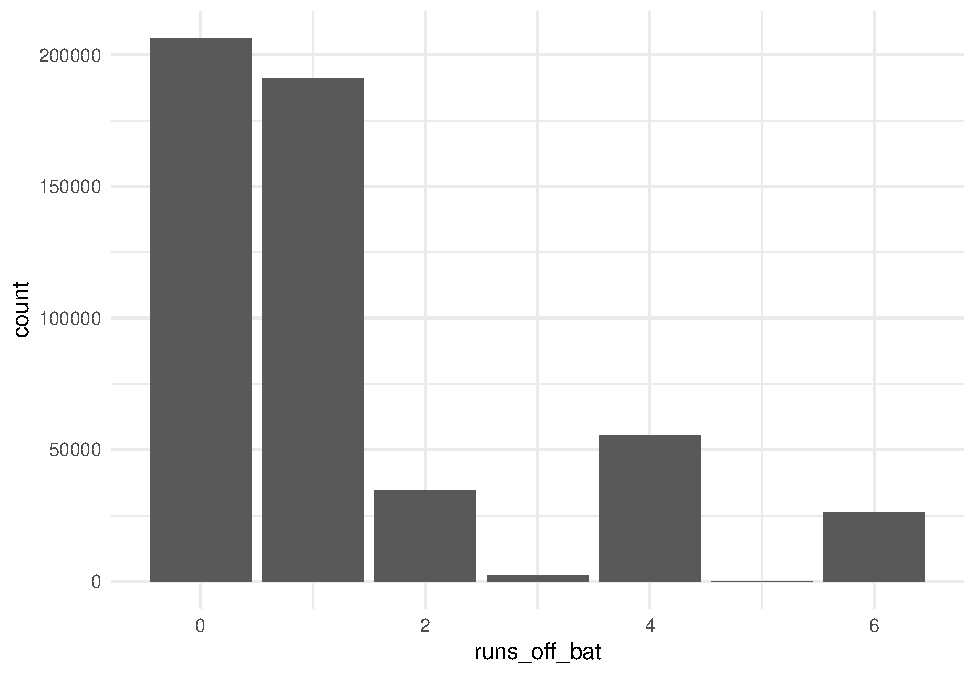
\includegraphics{paper_files/figure-latex/bar-1} 

}

\caption{Bar Plot of the number of runs scored of a particular pitch}\label{fig:bar}
\end{figure}

Figure \ref{fig:bar} shows a bar plot.

\hypertarget{sec:models}{%
\section{Models}\label{sec:models}}

Let \(r_i\) be the number of runs scored on the \(i\)-th ball with
\(i=1,\cdots,n\) and \(r_i \in \left\{0,1,\cdots,6\right\}\). Then
define \({\bf y_{i}} = \left(y_{i0},\ldots,y_{i6}\right)\) where
\(y_{ij} = I(r_i = j), \forall j = 0, \cdots, 6\) and \(I(.)\) is the
indicator function. We then model:

\[
{\bf y_i} \sim MN(1,{\bf p_i})
\] where \({\bf p_{i}} = \left(p_{i0},\ldots,p_{i6}\right)\), \(p_{ij}\)
is the probability that \(j\) runes are scored on the \(i\)-th ball, and
\(\sum_{j = 0}^{6} p_{ij} = 1\) for all \(i\).

\[
log\left(\frac{p_{j}}{p_{0}}\right) = \beta_{0j} + {\bf X}{\bf \beta}_j + b_{j,batter} + b_{j,bowler} + b_{j,runner}
\] for \(j = 1,\ldots,6\) where \(\beta_{0j}\) is the intercept of the
\(j\)-th linear component, \({\bf \beta}_j\) is a \(P\)-dimensional
vector containing the regression coefficients for the fixed effects,
\({\bf X}\) is the matrix of covariates, and
\(b_{j,batter}, b_{j,bowler}, b_{j,runner}\) are random effects for the
batter, bowler, and runner, respectively.

\hypertarget{priors}{%
\subsection{Priors}\label{priors}}

\(\beta_{j0} \sim N(0,1)\) for \(j = 1, \ldots, 6\) and
\(\beta_{jp} \sim N(0,1)\) for \(p = 1, \ldots, P\) and
\(j = 1, \ldots, 6\).

\(b_{j,batter} \sim N(0,\sigma^2_{batter})\) for all batters.
\(b_{j,bowler} \sim N(0,\sigma^2_{bowler})\) for all bowlers.
\(b_{j,runner} \sim N(0,\sigma^2_{runner})\) for all runners.

\(\sigma^2_{batter}, \sigma^2_{bowler}, \sigma^2_{runner} \sim Inv-\chi^2(something)\)

\hypertarget{sec:results}{%
\section{Results}\label{sec:results}}

\hypertarget{sec:conclusions}{%
\section{Discsusson, Future work and
conclusions}\label{sec:conclusions}}

\hypertarget{acknowledgements}{%
\section*{Acknowledgements}\label{acknowledgements}}
\addcontentsline{toc}{section}{Acknowledgements}

\hypertarget{supplementary-material}{%
\section*{Supplementary Material}\label{supplementary-material}}
\addcontentsline{toc}{section}{Supplementary Material}

All code for reproducing the analyses in this paper is publicly
available at \url{https://github.com/gjm112/cricketIPL}

\hypertarget{references}{%
\section{References}\label{references}}

\end{document}
